\documentclass[aspectratio=169]{beamer}
\usepackage[square,numbers]{natbib}
\bibliographystyle{apalike}
\title[Stibo Systems Case Presentation]{UX Architecture for Data Collaboration}
\date[]{\today}
\author[]{Henrik Korsgaard}
\institute{DEPARTMENT OF COMPUTER SCIENCE} % Type in A
\usetheme{henrikkorsgaard}

\usepackage{multicol}

\usetikzlibrary{shapes.geometric, shapes.symbols}
\usepackage{tikzpeople}
\usetikzlibrary{arrows.meta}
\usepackage{fontawesome5}
\usepackage{changepage}

\makeatletter
\newbox\@backgroundblock
\newenvironment{backgroundblock}[2]{%
  \global\setbox\@backgroundblock=\vbox\bgroup%
    \unvbox\@backgroundblock%
    \vbox to0pt\bgroup\vskip#2\hbox to0pt\bgroup\hskip#1\relax%
}{\egroup\egroup\egroup}
\addtobeamertemplate{background}{\box\@backgroundblock}{}
\makeatother

\makeatletter
    \newsavebox\restorebox
\newenvironment{restoretext}%
    {\@parboxrestore% 
     \begin{adjustwidth}{-8mm}{-8mm}%
                \begin{lrbox}{\restorebox}%
                \begin{minipage}{\linewidth}%
    }{\end{minipage}\end{lrbox}
        \usebox\restorebox
        \end{adjustwidth}
     }
\makeatother

\begin{document}

\begin{frame}
\maketitle
\end{frame}

\begin{frame}{Outline}
    \begin{columns}
        \begin{column}{0.5\textwidth}
            \begin{itemize}
                \item UX research process
                \item Results and observations
                \item Information design
                \item Interaction design
                %%\item If time, responsive filtering %% if you cannot execute this within time, then keep
            \end{itemize}
        \end{column}
        \begin{column}{0.5\textwidth}
            As a newly hired UX architect, your initial task is to create an outline for the UX work in a project aimed at improving the UX of the \textbf{collaboration tooling}\footnotemark{} in an existing online Excel-like table system.\\
            \vspace{1em}
            {\color{HenrikFontLight}\dots assume that you have the necessary budget for it.}
        \end{column}
    \end{columns}
    \footnotetext{Ida Larsen-Ledet, and Henrik Korsgaard. Territorial functioning in \textbf{collaborative writing}. CSCW 2019\\Ida Larsen-Ledet, Henrik Korsgaard, and Susanne Bødker. \textbf{Collaborative writing} across multiple artifact ecologies.CHI 2020}
\end{frame}

\begin{frame}{UX Research}
    \begin{description}
        \small
        \item[Discovery:] \textbf{Why}, how, and when do users collaborate?
        \item[Define:] What are the main user scenarios, information concepts and features?
        \item[Prototype:] \textit{Everything!}
        \item[Evaluate:] User testing and evaluation
        \item[Integrate:] Plan integration and delivery
    \end{description}
    \begin{restoretext}
    \begin{backgroundblock}{7mm}{50mm}
    \centering
    \resizebox{1\textwidth}{!}{%
    \begin{tikzpicture}

        \node[diamond,fill=HenrikDark!4, minimum width = 4.5cm, minimum height = 4.5cm] (d) at (1.1,1) {};
        \node[diamond,fill=HenrikDark!4, minimum width = 4.5cm, minimum height = 4.5cm] (d) at (5.5,1) {};

        \node[signal to=east, signal from=west,shape=signal, draw, minimum width = 2.15cm, minimum height = 0.5cm, fill=white] at (0.1,1) {\tiny Discover};
        \node[signal to=east, signal from=west, shape=signal, draw, minimum width = 2.3cm, minimum height = 0.5cm, fill=white] at (2.2,1) {\tiny Define};
        \node[signal to=east, signal from=west, shape=signal, draw, minimum width = 2.3cm, minimum height = 0.5cm, fill=white] at (4.37,1) {\tiny Prototype};
        \node[signal to=east, signal from=west, shape=signal, draw, minimum width = 2.3cm, minimum height = 0.5cm, fill=white] at (6.54,1) {\tiny Evaluate};
        \node[signal to=east, signal from=west, shape=signal, draw, minimum width = 2.3cm, minimum height = 0.5cm, fill=white] at (8.7,1) {\tiny Integrate}; 
    \end{tikzpicture}
    }
\end{backgroundblock}
\end{restoretext}
\end{frame}


\begin{frame}{UX Research}
    \begin{columns}[t]
        \begin{column}{0.5\textwidth}
            \small
            \textbf{Discover}
            \begin{enumerate}
                \item Contextual interviews and task sessions observations
                \item Internal/external research
                \item Analytics (?)
                \item Workshops (?)
            \end{enumerate}
        \end{column}
        \begin{column}{0.5\textwidth}
            \small
            \textbf{Define}
            \begin{itemize}
                \item Collaborative task objectives 
                \item Scenarios, personas and user journeys
                \item Information concepts and architecture
                \item UX quality criteria and KPIs
            \end{itemize}
        \end{column}
    \end{columns}
    \begin{restoretext}
    \begin{backgroundblock}{7mm}{50mm}
    \centering
    \resizebox{1\textwidth}{!}{%
    \begin{tikzpicture}

        \node[diamond,fill=HenrikDark!4, minimum width = 4.5cm, minimum height = 4.5cm] (d) at (1.1,1) {};
        \node[diamond,fill=HenrikDark!4, minimum width = 4.5cm, minimum height = 4.5cm] (d) at (5.5,1) {};

        \node[signal to=east, signal from=west,shape=signal, draw, minimum width = 2.15cm, minimum height = 0.5cm,white, fill=HenrikDark] at (0.1,1) {\tiny Discover};
        \node[signal to=east, signal from=west, shape=signal, draw, minimum width = 2.3cm, minimum height = 0.5cm,white,fill=HenrikDark] at (2.2,1) {\tiny Define};
        \node[signal to=east, signal from=west, shape=signal, draw, minimum width = 2.3cm, minimum height = 0.5cm] at (4.37,1) {\tiny Prototype};
        \node[signal to=east, signal from=west, shape=signal, draw, minimum width = 2.3cm, minimum height = 0.5cm, fill=white] at (6.54,1) {\tiny Evaluate};
        \node[signal to=east, signal from=west, shape=signal, draw, minimum width = 2.3cm, minimum height = 0.5cm, fill=white] at (8.7,1) {\tiny Integrate}; 
    \end{tikzpicture}
    }
\end{backgroundblock}
\end{restoretext}
\end{frame}

\begin{frame}{UX Research -- iterate where needed}
    \begin{columns}[t]
        \begin{column}{0.5\textwidth}
            \small
            \textbf{Prototype}
            \begin{itemize}
                \item User- and collaborative flow
                \item Information architecture and UI design
                \item Key interfaces and technical features
            \end{itemize}
        \end{column}
        \begin{column}{0.5\textwidth}
            \small
            \textbf{Evaluate}
            \begin{itemize}
                \item Internal review and testing
                \item User feedback (informal/think aloud)
                \item Review UX quality criteria and KPIs
            \end{itemize}
        \end{column}
    \end{columns}
    \begin{restoretext}
    \begin{backgroundblock}{7mm}{50mm}
    \centering
    \resizebox{1\textwidth}{!}{%
    \begin{tikzpicture}

        \node[diamond,fill=HenrikDark!4, minimum width = 4.5cm, minimum height = 4.5cm] (d) at (1.1,1) {};
        \node[diamond,fill=HenrikDark!4, minimum width = 4.5cm, minimum height = 4.5cm] (d) at (5.5,1) {};

        \node[signal to=east, signal from=west,shape=signal, draw, minimum width = 2.15cm, minimum height = 0.5cm] at (0.1,1) {\tiny Discover};
        \node[signal to=east, signal from=west, shape=signal, draw, minimum width = 2.3cm, minimum height = 0.5cm] at (2.2,1) {\tiny Define};
        \node[signal to=east, signal from=west, shape=signal, draw, minimum width = 2.3cm, minimum height = 0.5cm, white, fill=HenrikDark] at (4.37,1) {\tiny Prototype};
        \node[signal to=east, signal from=west, shape=signal, draw, minimum width = 2.3cm, minimum height = 0.5cm, white, fill=HenrikDark] at (6.54,1) {\tiny Evaluate};
        \node[signal to=east, signal from=west, shape=signal, draw, minimum width = 2.3cm, minimum height = 0.5cm, fill=white] at (8.7,1) {\tiny Integrate}; 
    \end{tikzpicture}
    }
\end{backgroundblock}
\end{restoretext}
\end{frame}

% \begin{frame}{Results: Collaborative scenarios}
%     \begin{columns}
%         \begin{column}{0.7\textwidth}
%             \small
%             \textbf{Collaboration projects}
%             \begin{itemize}
%                 \footnotesize
%                 \item Multiple peers collaborate on a larger task over time
%                 \item Different roles, responsibilities and expertise
%                 \item Turn-taking with a high degree of coordination
%             \end{itemize}
%             \textbf{Incident response}
%             \begin{itemize}
%                 \footnotesize
%                 \item 2 peers collaborate to solve a pressing issue
%                 \item Real-time ``jump-in-and-consult'' collaboration
%             \end{itemize}
%             \textbf{Training}
%             \begin{itemize}
%                 \footnotesize
%                 \item Instructor help one or more trainees
%                 \item Focused on learning the application and/or data 
%             \end{itemize}
%         \end{column}
%         \begin{column}{0.3\textwidth}
%             \centering
%             \resizebox{0.8\textwidth}{!}{%
%             \begin{tikzpicture}
%                 \node[] at (0,2.1) {\small\faUser};
%                 \draw[{Straight Barb[scale=0.5]}-{Straight Barb[scale=0.5]}] (0.25,2) to[bend right=-45] (0.58,1.5);
%                 \node[] at (0.55,1.2) {\small\faUser};
%                 \draw[{Straight Barb[scale=0.5]}-{Straight Barb[scale=0.5]}] (-0.25,2) to[bend right=45] (-0.58,1.5);
%                 \node[] at (0,1.5) {\scriptsize\faDatabase};
%                 \draw[{Straight Barb[scale=0.5]}-{Straight Barb[scale=0.5]}] (-0.3,1) to[bend right=45] (0.3,1);
%                 \node[] at (-0.55,1.2) {\small\faUser};

%                 \node[] at (0.7,0) {\small\faUser};
%                 \draw[{Straight Barb[scale=0.5]}-] (0.15,0) to (0.5,0);
%                 \node[] at (0,0) {\tiny\faDatabase};
%                 \draw[{Straight Barb[scale=0.5]}-] (-0.15,0) to (-0.5,0);
%                 \node[] at (-0.7,0) {\small\faUser};

%                 \node[] at (-0.7,-1.5) {\small\faUser};
%                 \draw[-{Straight Barb[scale=0.5]}] (-0.5,-1.5) to (-0.15,-1.5);
%                 \node[] at (0,-1.5) {\tiny\faDatabase};
%                 \draw[-{Straight Barb[scale=0.5]}] (0.15,-1.4) to (0.5,-1.1);
%                 \draw[-{Straight Barb[scale=0.5]}] (0.15,-1.5) to (0.5,-1.5);
%                 \draw[-{Straight Barb[scale=0.5]}] (0.15,-1.6) to (0.5,-1.9);
%                 \node[] at (0.7,-1.1) {\scriptsize\faUser};
%                 \node[] at (0.7,-1.5) {\scriptsize\faUser};
%                 \node[] at (0.7,-1.9) {\scriptsize\faUser};
%             \end{tikzpicture}
%             }
%         \end{column}
%     \end{columns}
% \end{frame}

\begin{frame}{Results: Collaborative scenarios}
    \setlength{\leftmargini}{0.5cm}
    \begin{columns}[t]
        \begin{column}{0.33\textwidth}
            \textbf{\small 1. Collaborative projects}
            \begin{itemize}
                \scriptsize
                \item Peers collaborate on a larger project
                \item Different responsibilities and expertise
                \item Mixed focus collaboration with a high degree of coordination
                \item Multiple data views
            \end{itemize}
        \end{column}
        \begin{column}{0.33\textwidth}
            \textbf{\small 2. Real-time collaboration}
            \begin{itemize}
                \scriptsize
                \item Peers collaborate on smaller (urgent) tasks
                \item Real-time collaboration
                \item Shared task focus 
                \item Few data views
            \end{itemize}
        \end{column}
        \begin{column}{0.33\textwidth}
            \textbf{\small 3. Training}
            \begin{itemize}
                \scriptsize
                \item Expert user provide training and onboarding of novices
                \item Focused on learning the application and/or data
                \item Tailored data views and exercises
            \end{itemize}
        \end{column}
    \end{columns}
\end{frame}

\begin{frame}{Results: Key UX qualities}
    \begin{columns}
        \begin{column}{0.6\textwidth}
            \small
            \begin{itemize}
                \item Sharing with collaborators should be easy and include task assignment and notes
                \item Important to know who did what in a shared view (awareness, track changes, accountability etc.)
                \item Support sandbox experimentation and analysis before publishing
                \item Collaborative features should not overshadow existing task features
                %\item A majority mention Google Drive as an example of a great collaboration tool
            \end{itemize}
        \end{column}
        \begin{column}{0.4\textwidth}
            \begin{figure}[h]
                \centering
                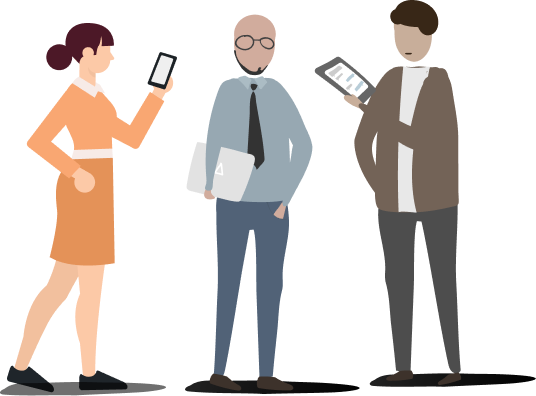
\includegraphics[width=1\textwidth]{images/Users.png}
            \end{figure}
        \end{column}
    \end{columns}
\end{frame}

\begin{frame}{Results: State-of-the-art collaborative UX}
    \begin{columns}
        \begin{column}{0.6\textwidth}
            \begin{itemize}
                \small
                \item Work object is shared by replication (content and formatting)
                \item Communication is transient (chat)
                \item Tools are individual, but similar across users (`what-you-see-I-see')
                \item Environment is not shared (browser/extensions)
                \item[]
                \item Not perfect, e.g. `the jumping text problem' and `cursor wars'
            \end{itemize}
        \end{column}
        \begin{column}{0.4\textwidth}
            \begin{figure}[h]
                \centering
                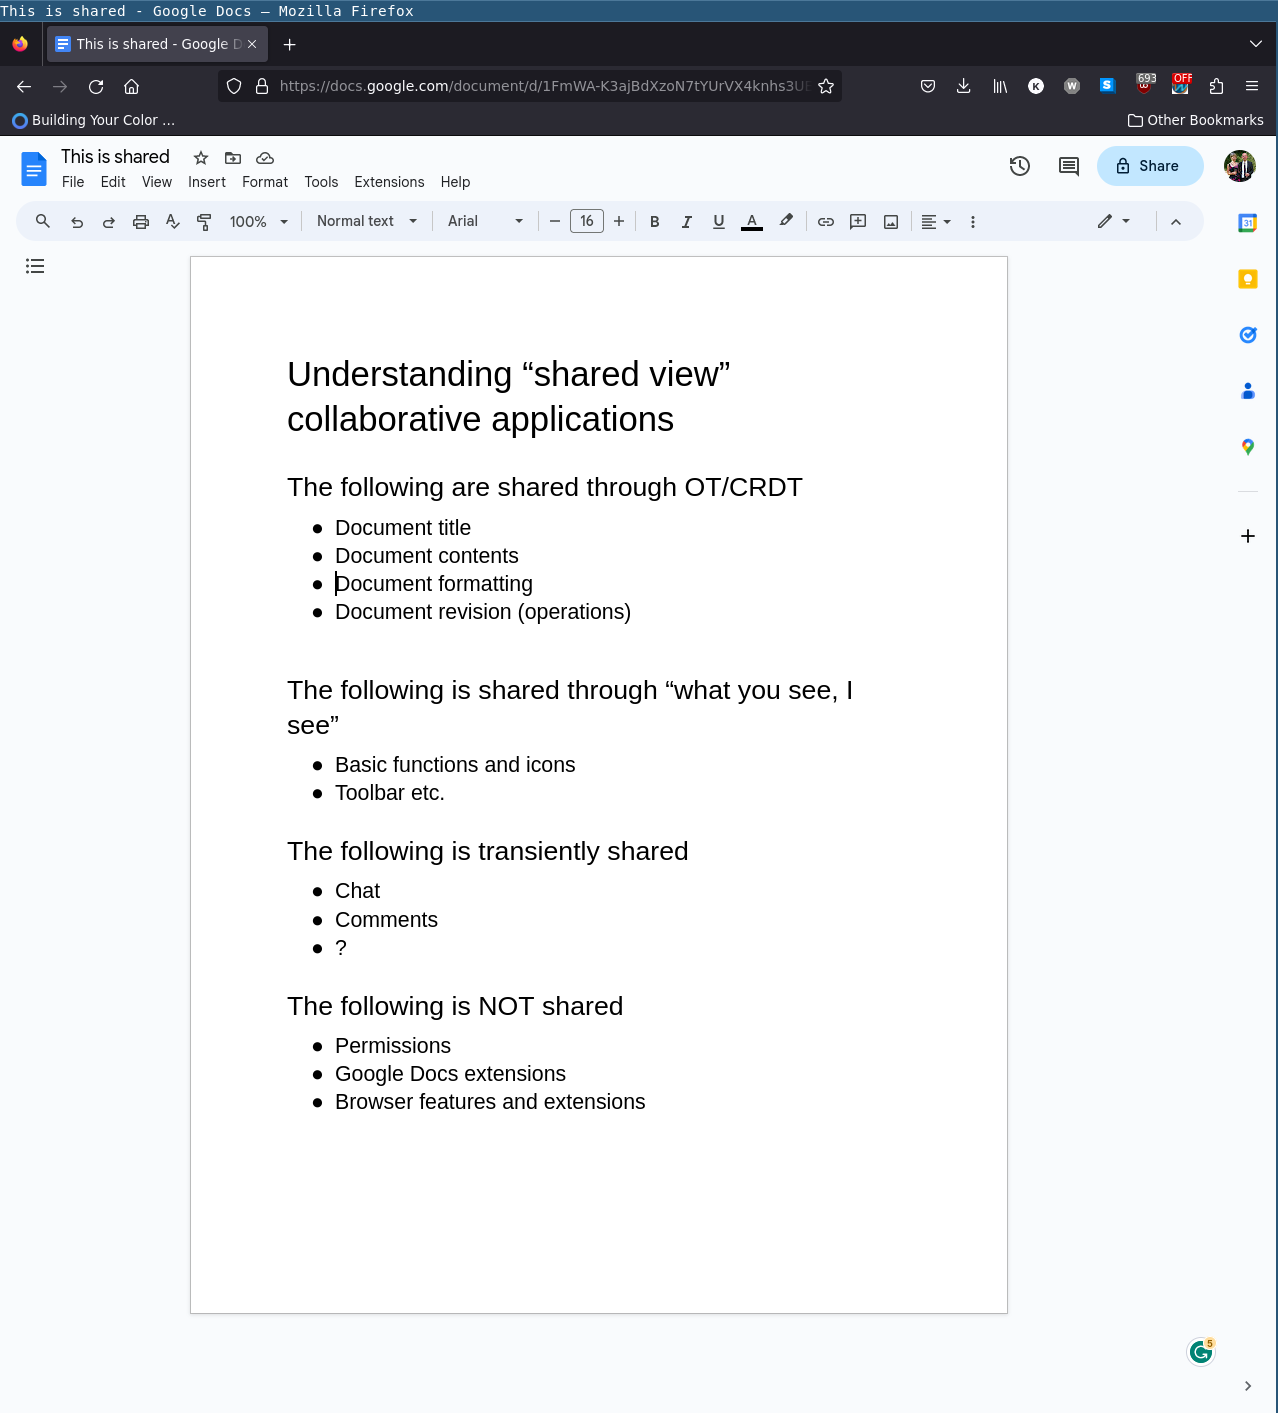
\includegraphics[width=1\textwidth]{images/gdocs.png}
                %\caption{Google Documents Sharing Model}
            \end{figure}
        \end{column}
    \end{columns}
\end{frame}

\begin{frame}{Interaction Design features}
    \begin{itemize}
        \item The user can save changes as individual \textbf{views} (sheets) of data
        \item \textbf{The user can share their saved views with other users}
        \item[] $\rightarrow$ The user can add or remove columns from the \textbf{view}
        \item[] $\rightarrow$ Users can filter and order the table content
        \item \textbf{Multiple users must be able to work on the same views simultaneously}
        \item[] $\rightarrow$ The users of the system may be located on multiple locations
    \end{itemize} 
\end{frame}


\begin{frame}{Making data views first class objects}
    \begin{columns}
        \begin{column}{0.4\textwidth}
            %% sige noget om hvorfor det er en challenge
            \begin{itemize}
                \footnotesize
                \item Data views are the main work objects -- they are what we share when collaborating
                \item Views can be published in formats fitting the consumer needs
                \item A data view encapsulate a data source, users, and the revision history
            \end{itemize}
        \end{column}
        \begin{column}{0.6\textwidth}
            \begin{figure}[h]
                \centering
                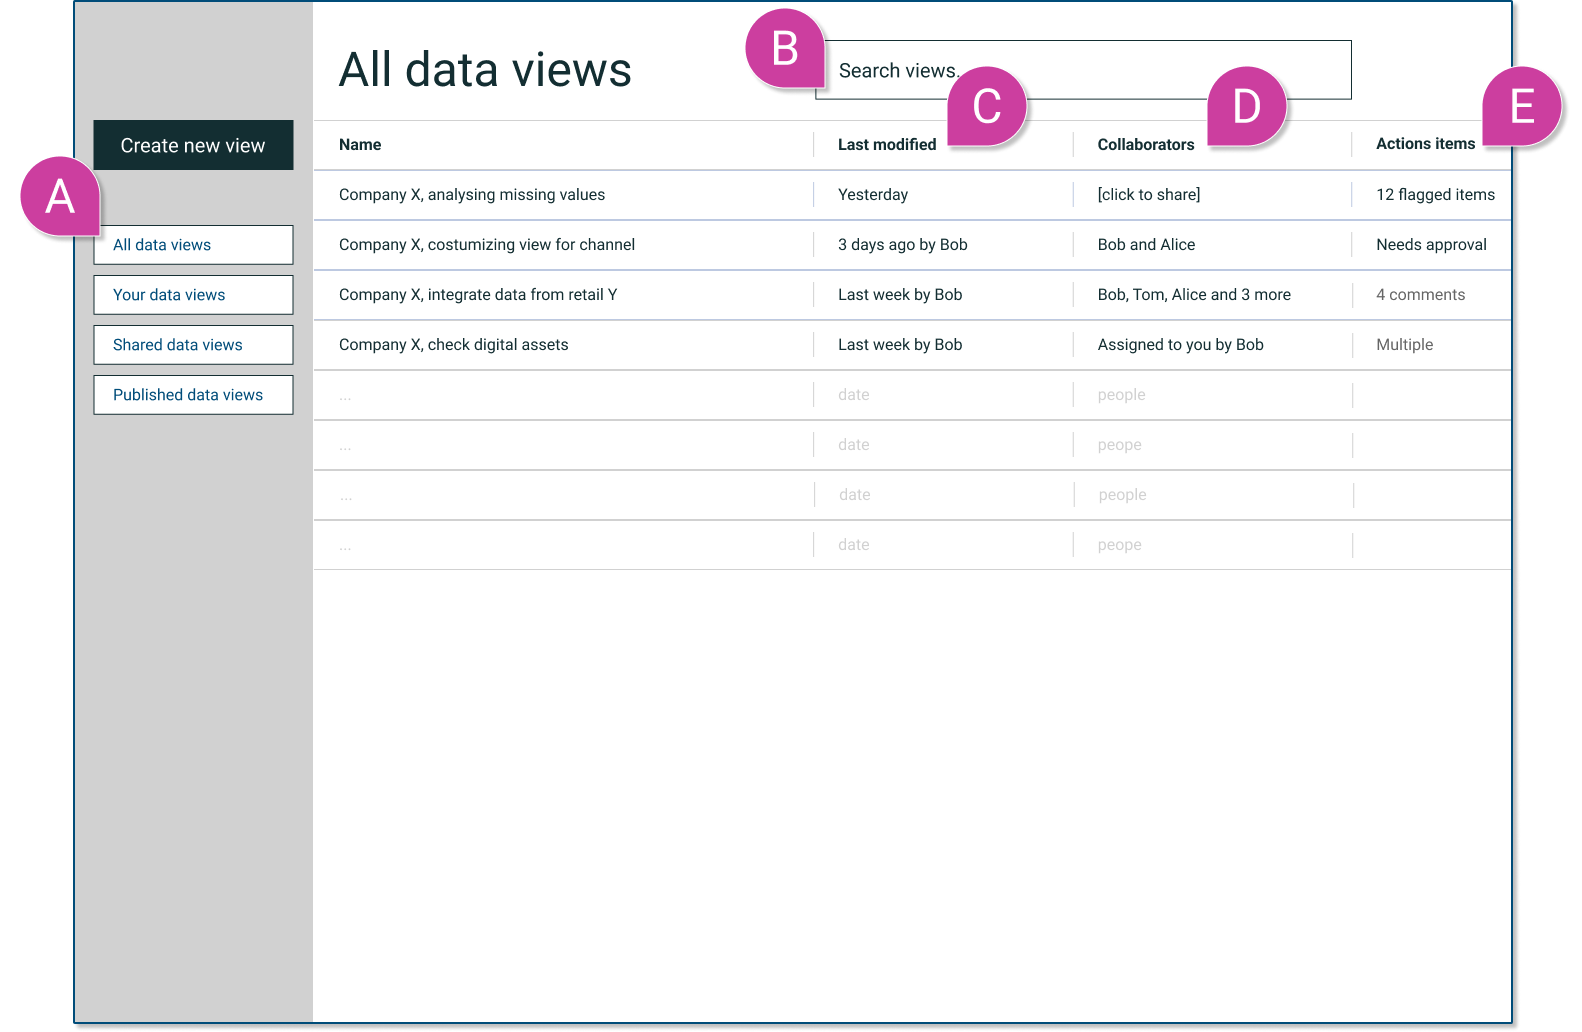
\includegraphics[width=1.1\textwidth]{images/all-views-with-marks.png}
            \end{figure}
        \end{column}
    \end{columns}
\end{frame}

\begin{frame}{Creating a new data view}
    \begin{figure}[h]
        \centering
        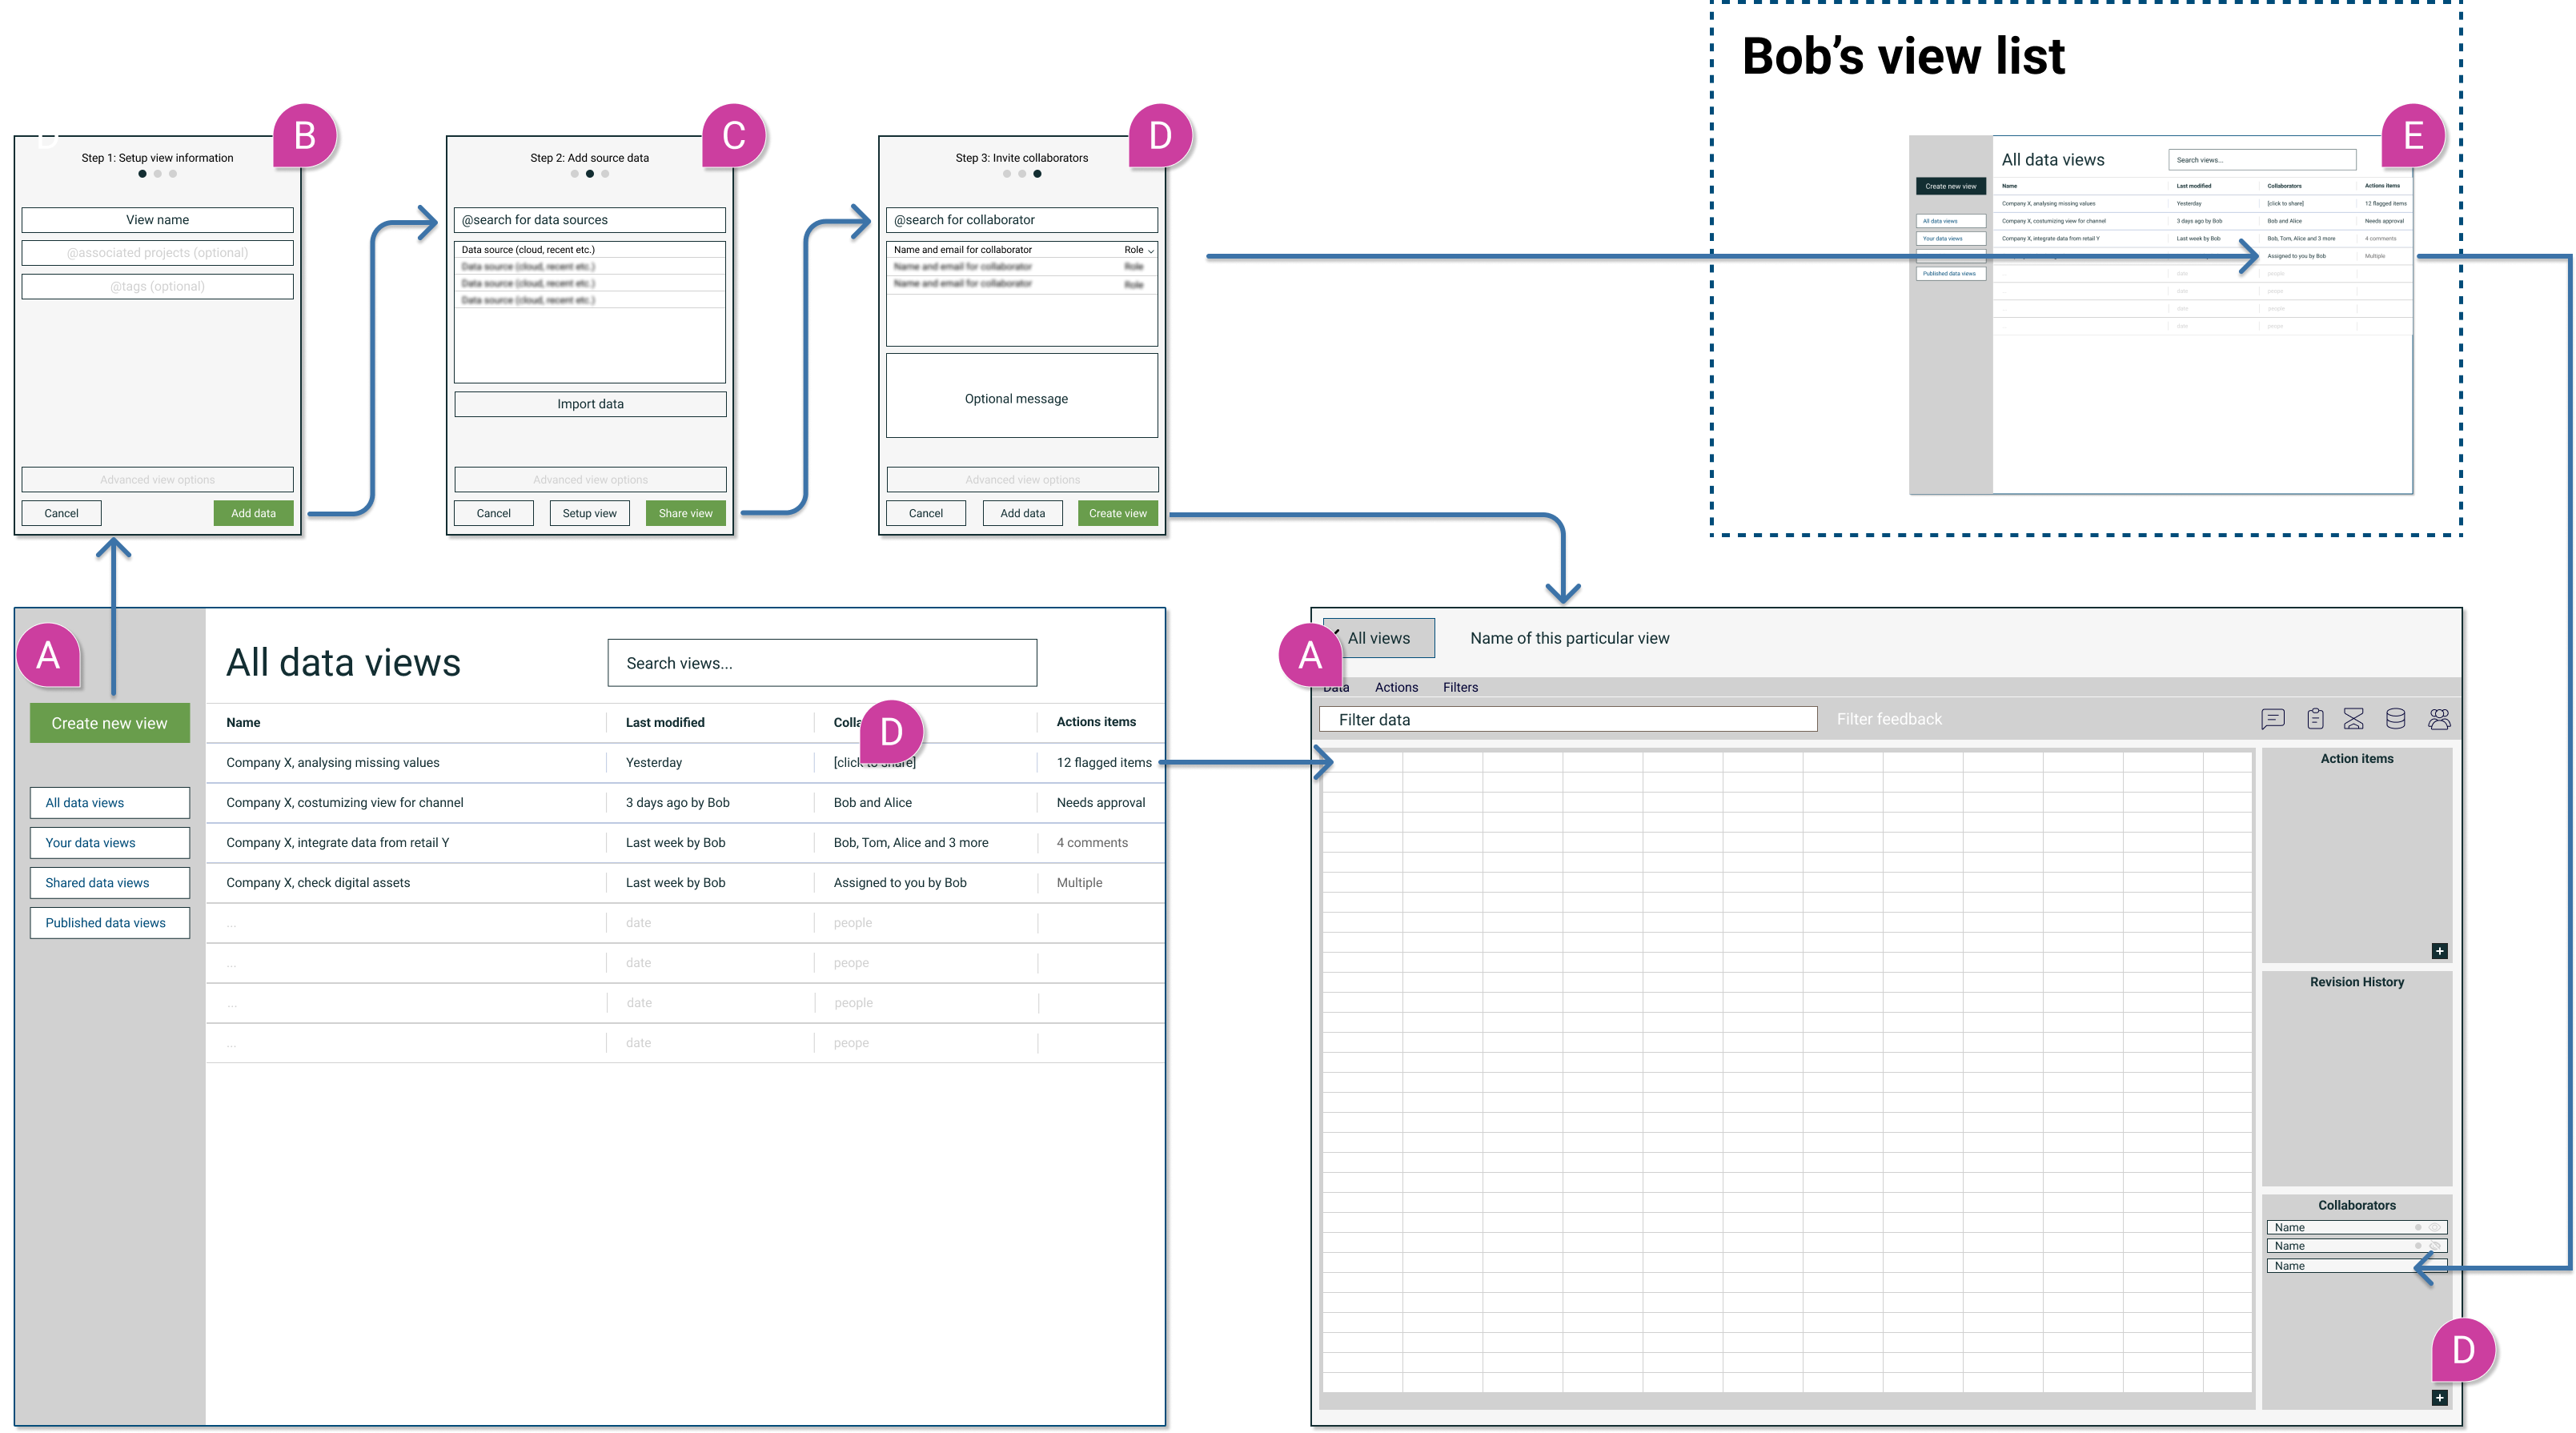
\includegraphics[width=1\textwidth]{images/create-new-view-flow.png}
    \end{figure}
\end{frame}

\begin{frame}{Collaborative tooling with tabular data}
    \begin{columns}
        \begin{column}{0.4\textwidth}
            %% sige noget om hvorfor det er en challenge
            \begin{itemize}
                \small
                \item Tabular view is the primary synchronized/shared object
                \item \dots filters cannot be shared until operationalized
                \begin{itemize}
                    \scriptsize
                    \vspace{0.4em}
                    \item \textbf{Action items} to support different roles
                    \vspace{0.2em}
                    \item \textbf{History} to support track changes and accountability
                    \vspace{0.2em}
                    \item \textbf{Collaborator} pane for navigation, awareness and mute
                \end{itemize}
            \end{itemize}
        \end{column}
        \begin{column}{0.6\textwidth}
            \begin{figure}[h]
                \centering
                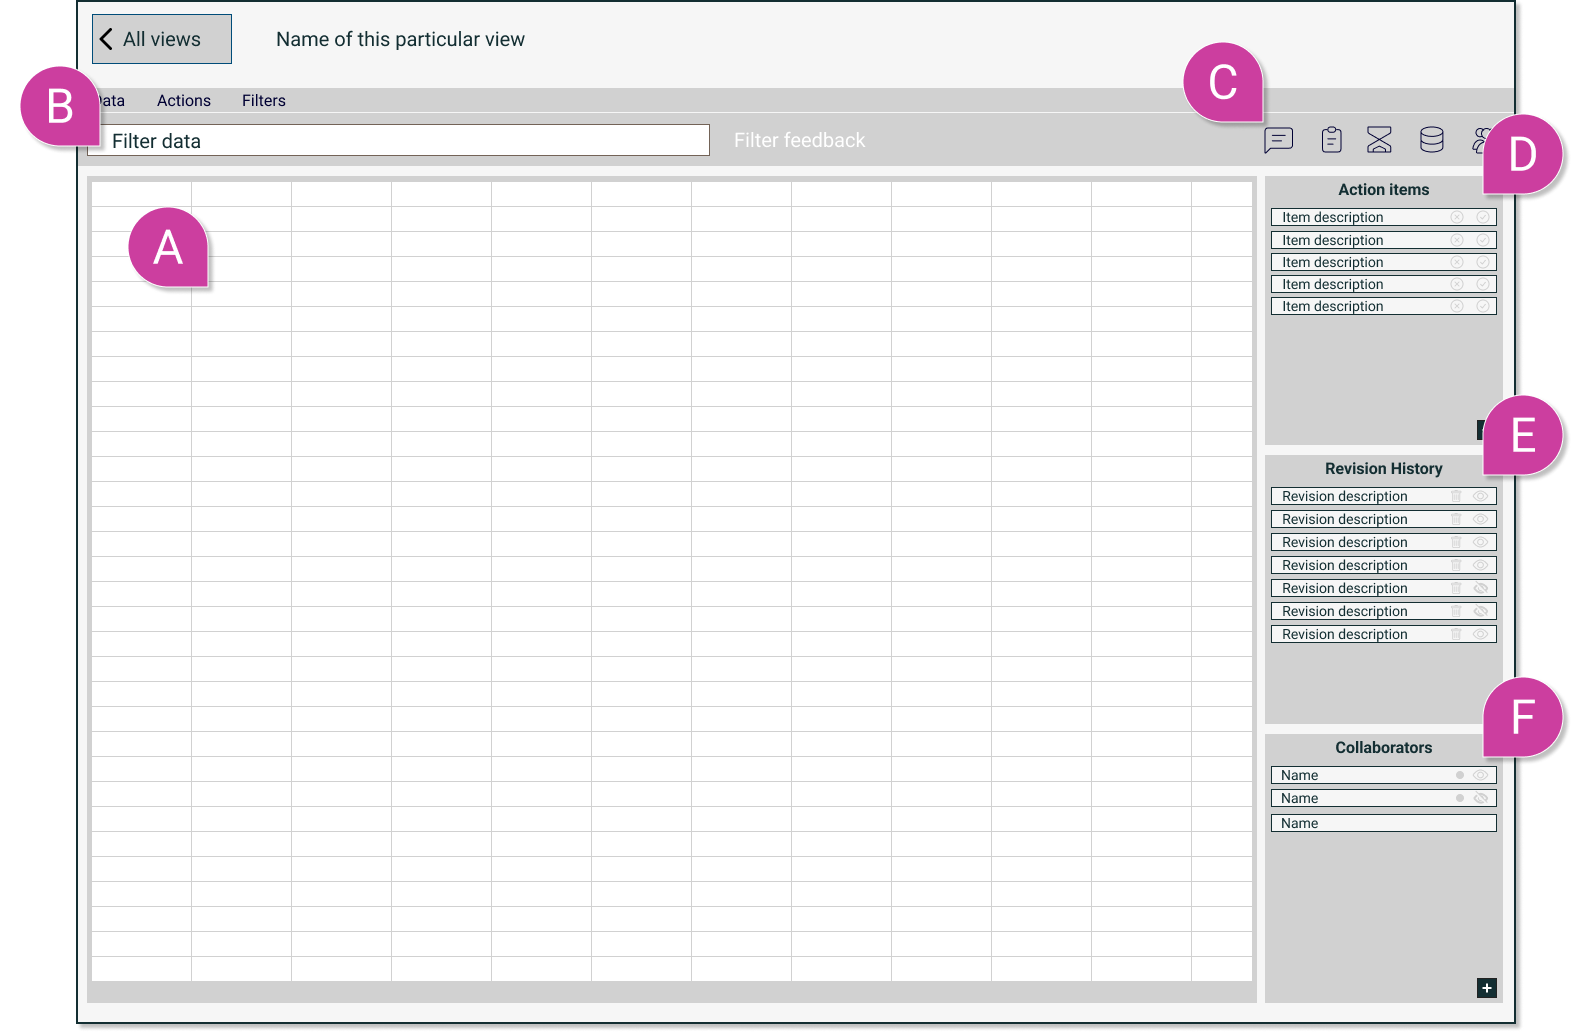
\includegraphics[width=1\textwidth]{images/filter-view-with-marks.png}
            \end{figure}
        \end{column}
    \end{columns}
\end{frame}

%% introduce the view design slide

\begin{frame}{Revision history as key\\ collaboration support}
    \begin{columns}
        \begin{column}{0.5\textwidth}
            \begin{itemize}
                \small
                \item Data operations as the replicated objects (CRDT)
                \item Support task resumption, accountability and finding stuff
                \item Support experimentation -- you can always roll back changes
                \item A set of operations can be applied to other data views (macros)
            \end{itemize}
        \end{column}
        \begin{column}{0.5\textwidth}
            \begin{figure}[h]
                \vspace{-4em}
                \centering
                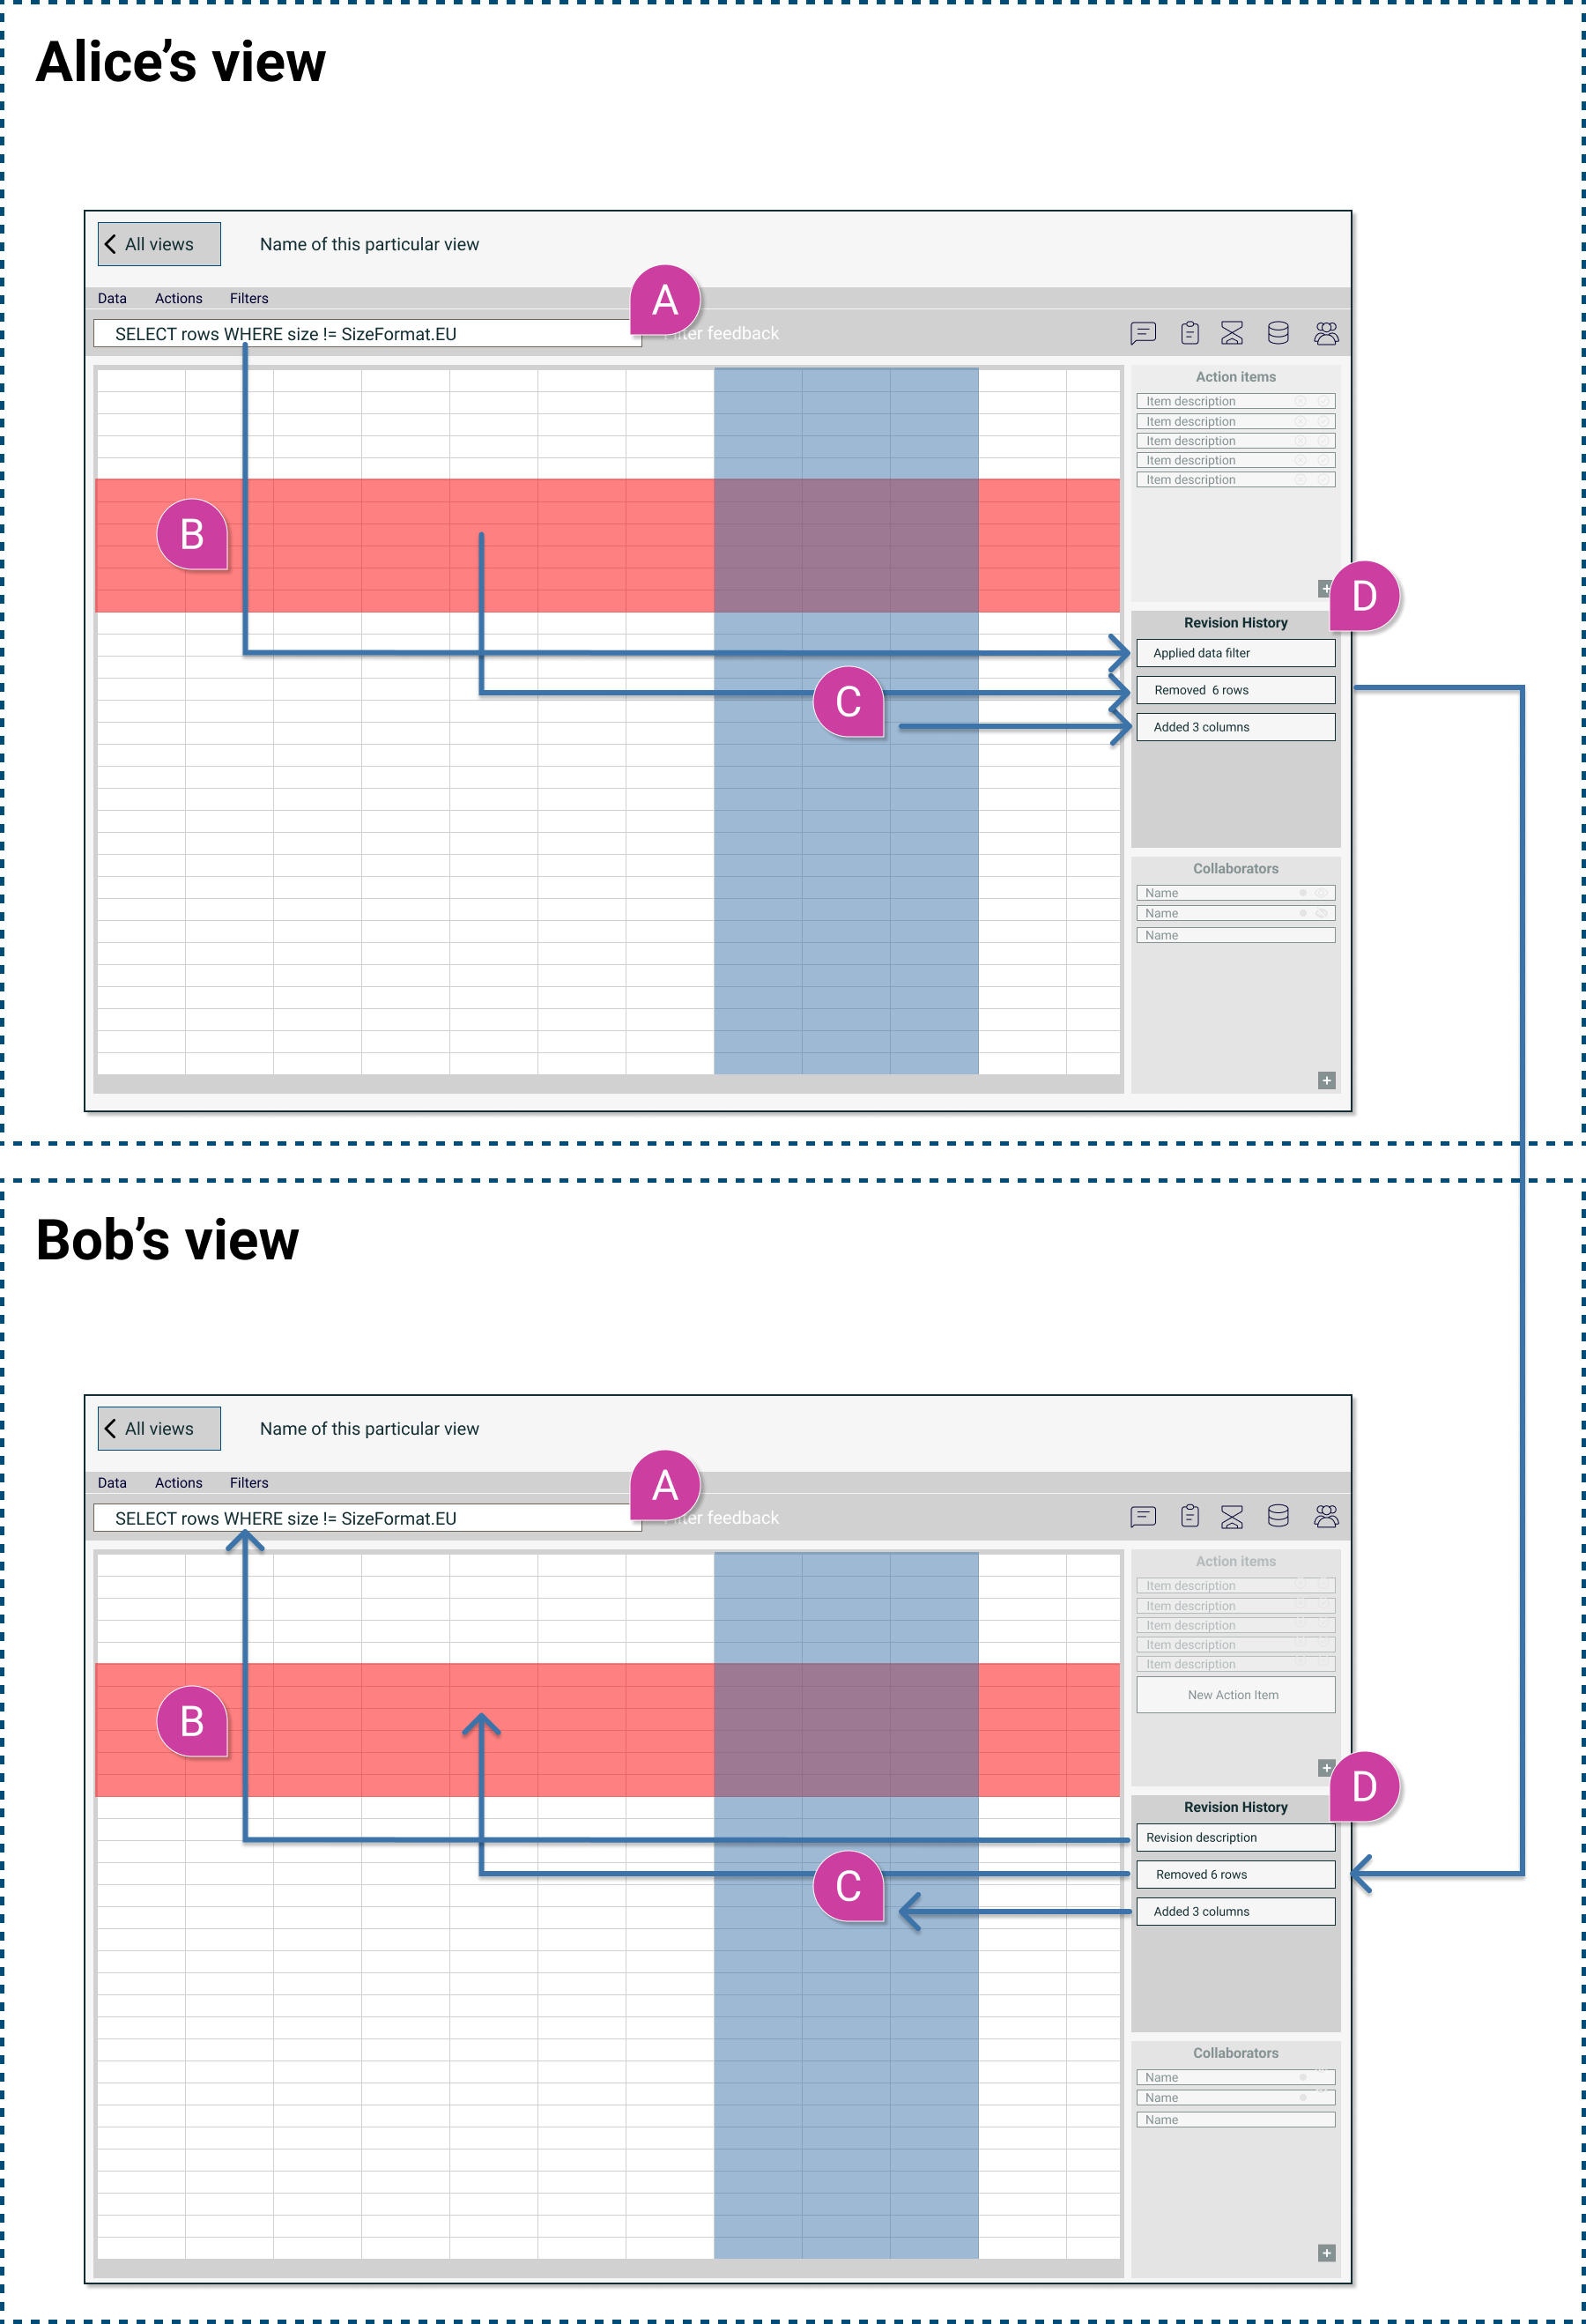
\includegraphics[width=0.9\textwidth]{images/shared-history.png}
            \end{figure}
        \end{column}
    \end{columns}
\end{frame}

\begin{frame}{Collaborating on common tasks: Assign action item}
    \vspace{2em}
    \begin{restoretext}
    \begin{figure}[h]
        \centering
        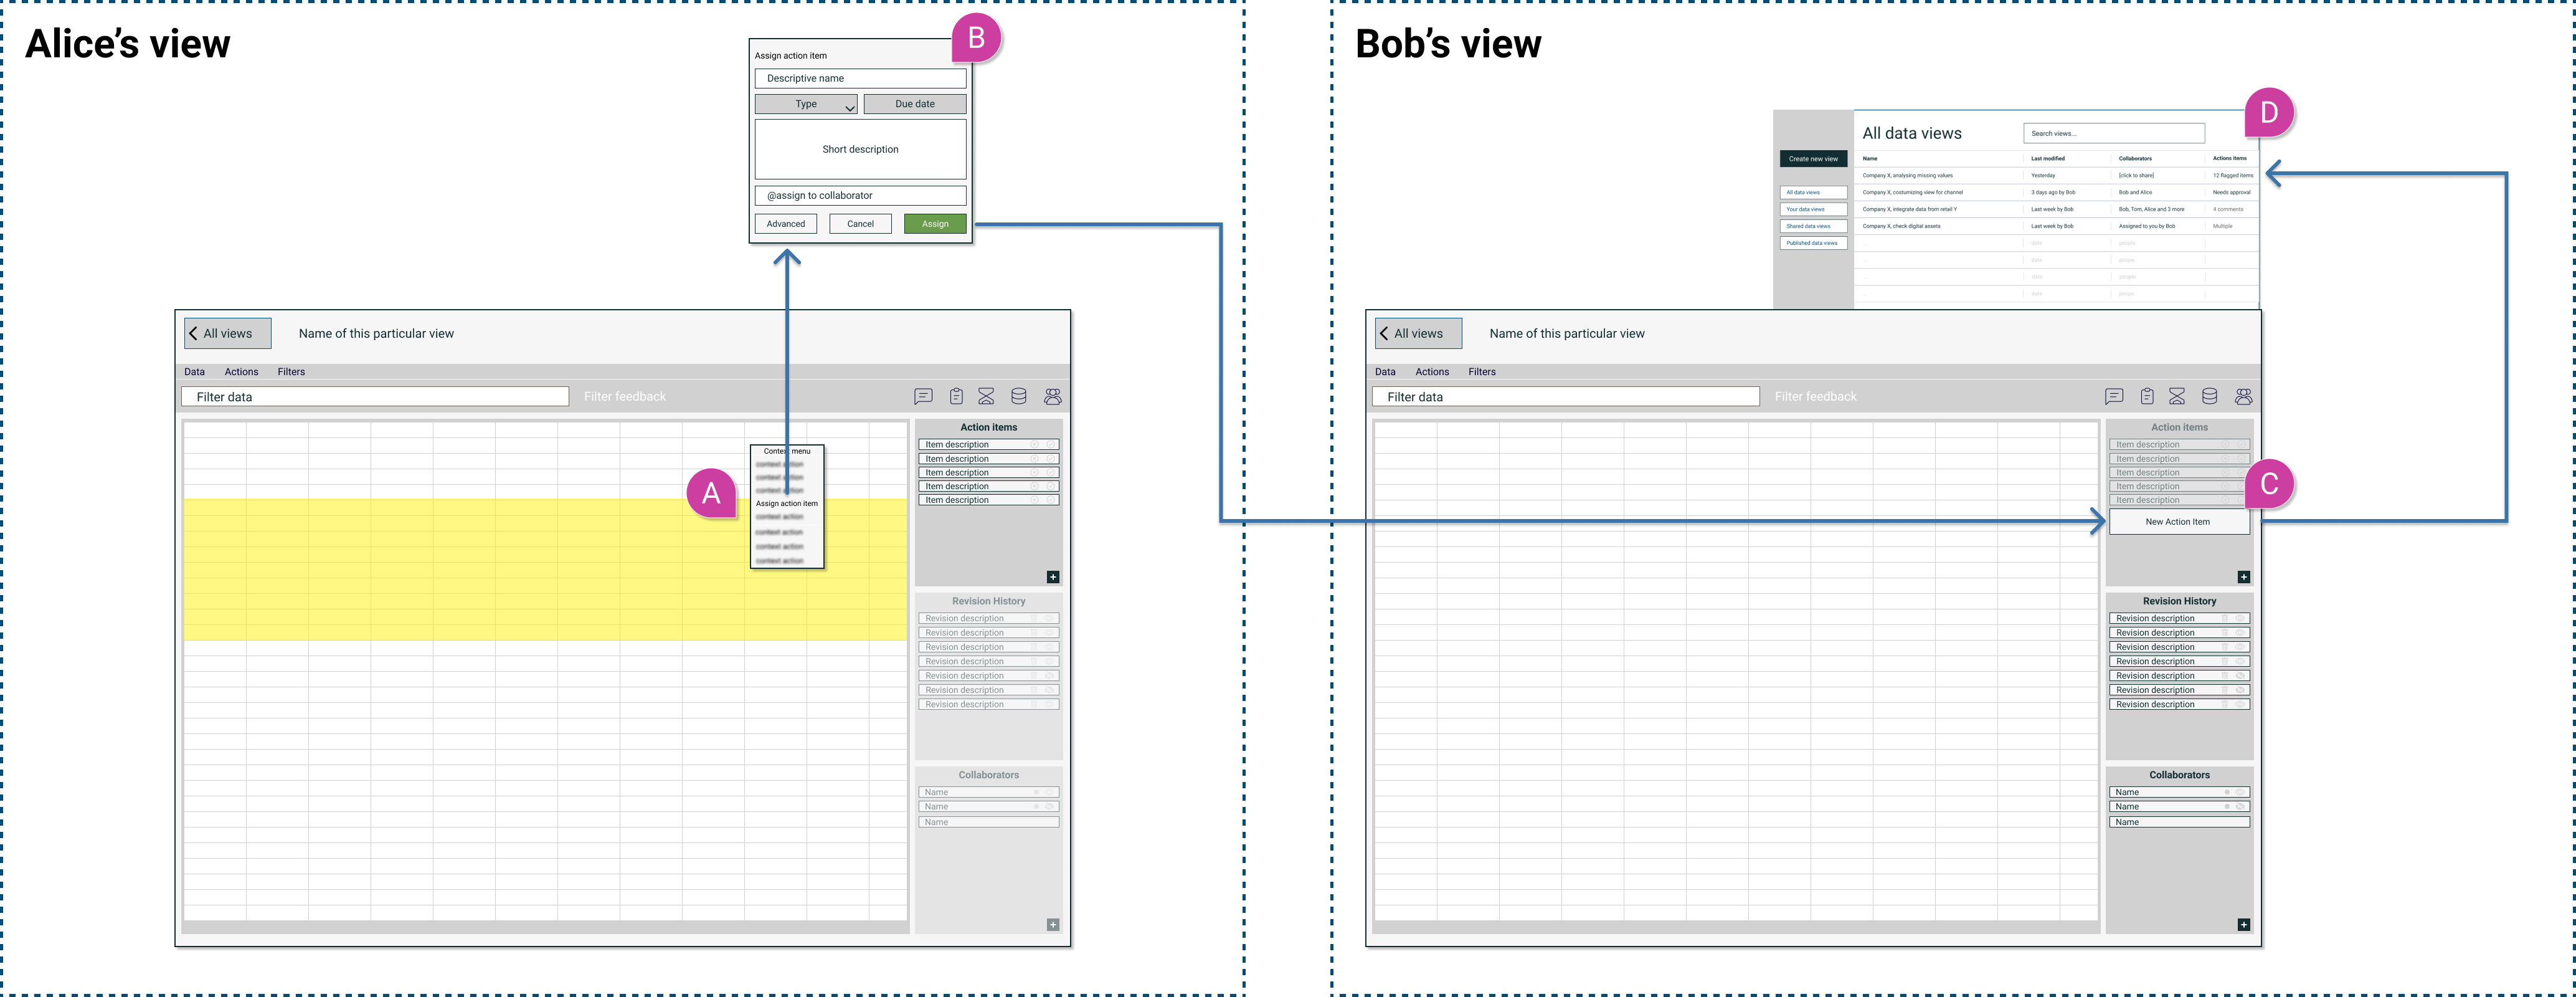
\includegraphics[width=1\textwidth]{images/assign-action-item.png}
    \end{figure}
\end{restoretext}
\end{frame}

%% Skip if needed
% \begin{frame}{Key IA/IxD challenges}
%     \setlength\itemsep{10em}
%     \begin{itemize}
%         \item `Views' might be a difficult concept to grasph 
%         \item Revision history is powerful tool, but difficult to get right 
%         \item Remote collaboration \textbf{require} additional communication channels
%         \item Developing and prototyping collaborative features pose different requirements than single user applications:
%         \begin{itemize}
%             \footnotesize
%             \vspace{0.3em}
%             \item Require more contextual user research and co-design activities
%             \vspace{0.1em}
%             \item Hard to study from application analytics
%             \vspace{0.1em}
%             \item Require some technical infrastructure to prototype collaboration
%         \end{itemize}
%     \end{itemize}
% \end{frame}

\begin{frame}[DarkSlide]{}
    \vspace{3em}
    \centering
    \Large THANK YOU\\
\end{frame}

\end{document}